% !TEX root = main.tex

\section{线程}
在没有线程概念的系统中,进程是\textbf{资源分配}、调度/执行的单位;而在有线程概念的系统中,线程就成了\textbf{基本调度单位}/程序执行流最小单元,由线程ID、程序计数器、寄存器集合和堆栈组成。

线程独立拥有寄存器和栈等现场状态,只会与进程共享地址空间、代码和IO文件资源,\textbf{不与进程共享上下文寄存器}。

线程的优点:
\begin{itemize}
    \item 创建速度快
    \item 终止所用时间少
    \item 切换时间少
    \item 通信效率高,同一进程无需调用内核,共享存储空间
\end{itemize}

\bigskip
用户级线程(ULT):线程管理都由应用程序完成(线程库),内核不知道线程的存在,优点:
\begin{itemize}
    \item 线程切换不需要模式切换
    \item 调度算法可以应用程序专用
    \item ULT不需要内核支持,线程库可以在任何OS上运行
\end{itemize}
缺点:
\begin{itemize}
    \item 一个线程阻塞会导致整个进程阻塞(因用户级线程对操作系统不可见,操作系统对整个进程进行调度)
    \item 不能利用多核和多处理器技术
\end{itemize}

\bigskip
内核级线程(KLT):线程管理由内核完成(提供API),调度基于线程进行,优点:
\begin{itemize}
    \item 线程阻塞不会导致进程阻塞
    \item 可以利用多核和多处理器技术
    \item 内核例程本身也可以使用多线程
\end{itemize}
缺点:
\begin{itemize}
    \item 线程切换需要进行模式切换
\end{itemize}

\bigskip
多线程模型
\begin{itemize}
    \item 多对一:多个用户级线程映射到一个内核级线程,线程管理在用户空间进行,效率高;若内核服务阻塞,则整个进程被阻塞
    \item 一对一:每个用户级线程映射到一个内核级线程,开销大
    \item 多对多:折中
\end{itemize}
\begin{figure}[H]
    \centering
    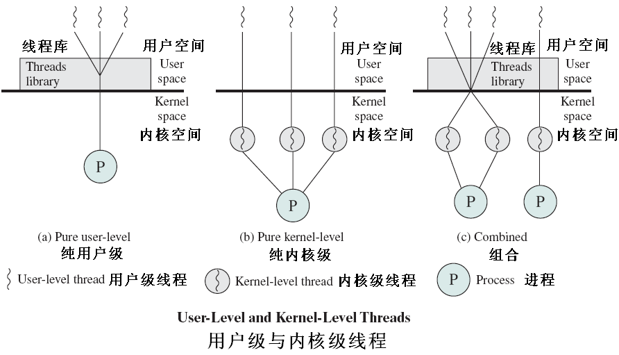
\includegraphics[width=0.6\linewidth]{fig/threads.png}
\end{figure}

线程与进程之间的关系
\begin{itemize}
    \item 1:1,每个进程都有唯一线程,DOS、传统Unix
    \item M:1,一个进程多个线程,Windows NT、Linux、Mac OS、iOS
    \item 1:M,一个线程可在多个进程环境中迁移
\end{itemize}

* Linux并不区分线程和进程,采用Copy On Write (COW)方式